\chapter{Project Methodology}
 \section{Software Development Model}
 The Agile model is an adaptable and iterative software development process that puts the needs of the client and flexibility first. It breaks the project up into manageable chunks known as sprints or iterations, enabling regular review and modification. Close collaboration between cross-functional teams results in functional software at the conclusion of each iteration. This cycle of iteration guarantees prompt reaction to evolving needs, promoting ongoing enhancement and contentment for the client. The Agile Manifesto's concepts of agile development include a strong emphasis on people and their relationships, functional software, customer collaboration, and adapting to change. In dynamic development contexts, the Agile approach has gained widespread adoption as a framework that encourages efficiency and reactivity.
 \begin{figure}[h]
	\centering
	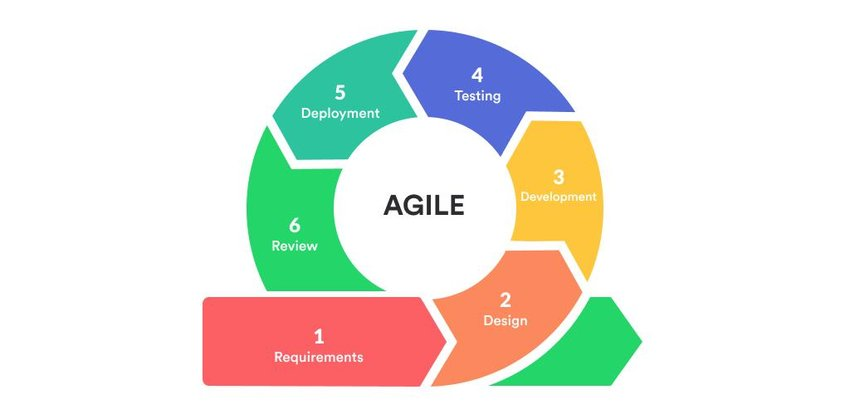
\includegraphics[scale=0.6]{images/Agile_model.png}
	\caption{Agile Model}
	
	\end{figure}
	
\pagebreak

	
	
	

\section{Description of working flow of proposed system}
\begin{enumerate}
	\item \textbf{Input (Video Frames):}
	\\ The input for a lip reading system typically consists of sequences of video frames, where each frame captures the movement and shape of the speaker's lips over time. The primary input is a video recording of a person speaking. Generally,the video contains a sequence of frames, each showing the speaker's lips in different positions.The video is processed to extract individual frames. The number of frames per second (fps) is a crucial parameter that influences the temporal resolution of the input data. Higher fps values can capture more detailed lip movements. The input video for this project has 25fps (frames per second).
	\item \textbf{Pre-processing:}
	\\Preprocessing in the context of a lip reading system involves a series of steps applied to the input video frames to enhance their quality, reduce noise, and ensure consistency. Typically, these steps aim to create a standardized and more informative input for the neural network.Normalization and enhancement techniques may be applied to the frames. This could include color normalization, resizing, or other transformations to ensure consistency and improve the model's robustness to variations in lighting and camera settings.The purpose of preprocessing is to prepare frames for optimal model input.Overall, preprocessing plays a crucial role in optimizing the input data, enabling the lip reading model to better learn and interpret the temporal and spatial features of lip motion.

	% \break
	
	\begin{figure}[h]
	\centering
	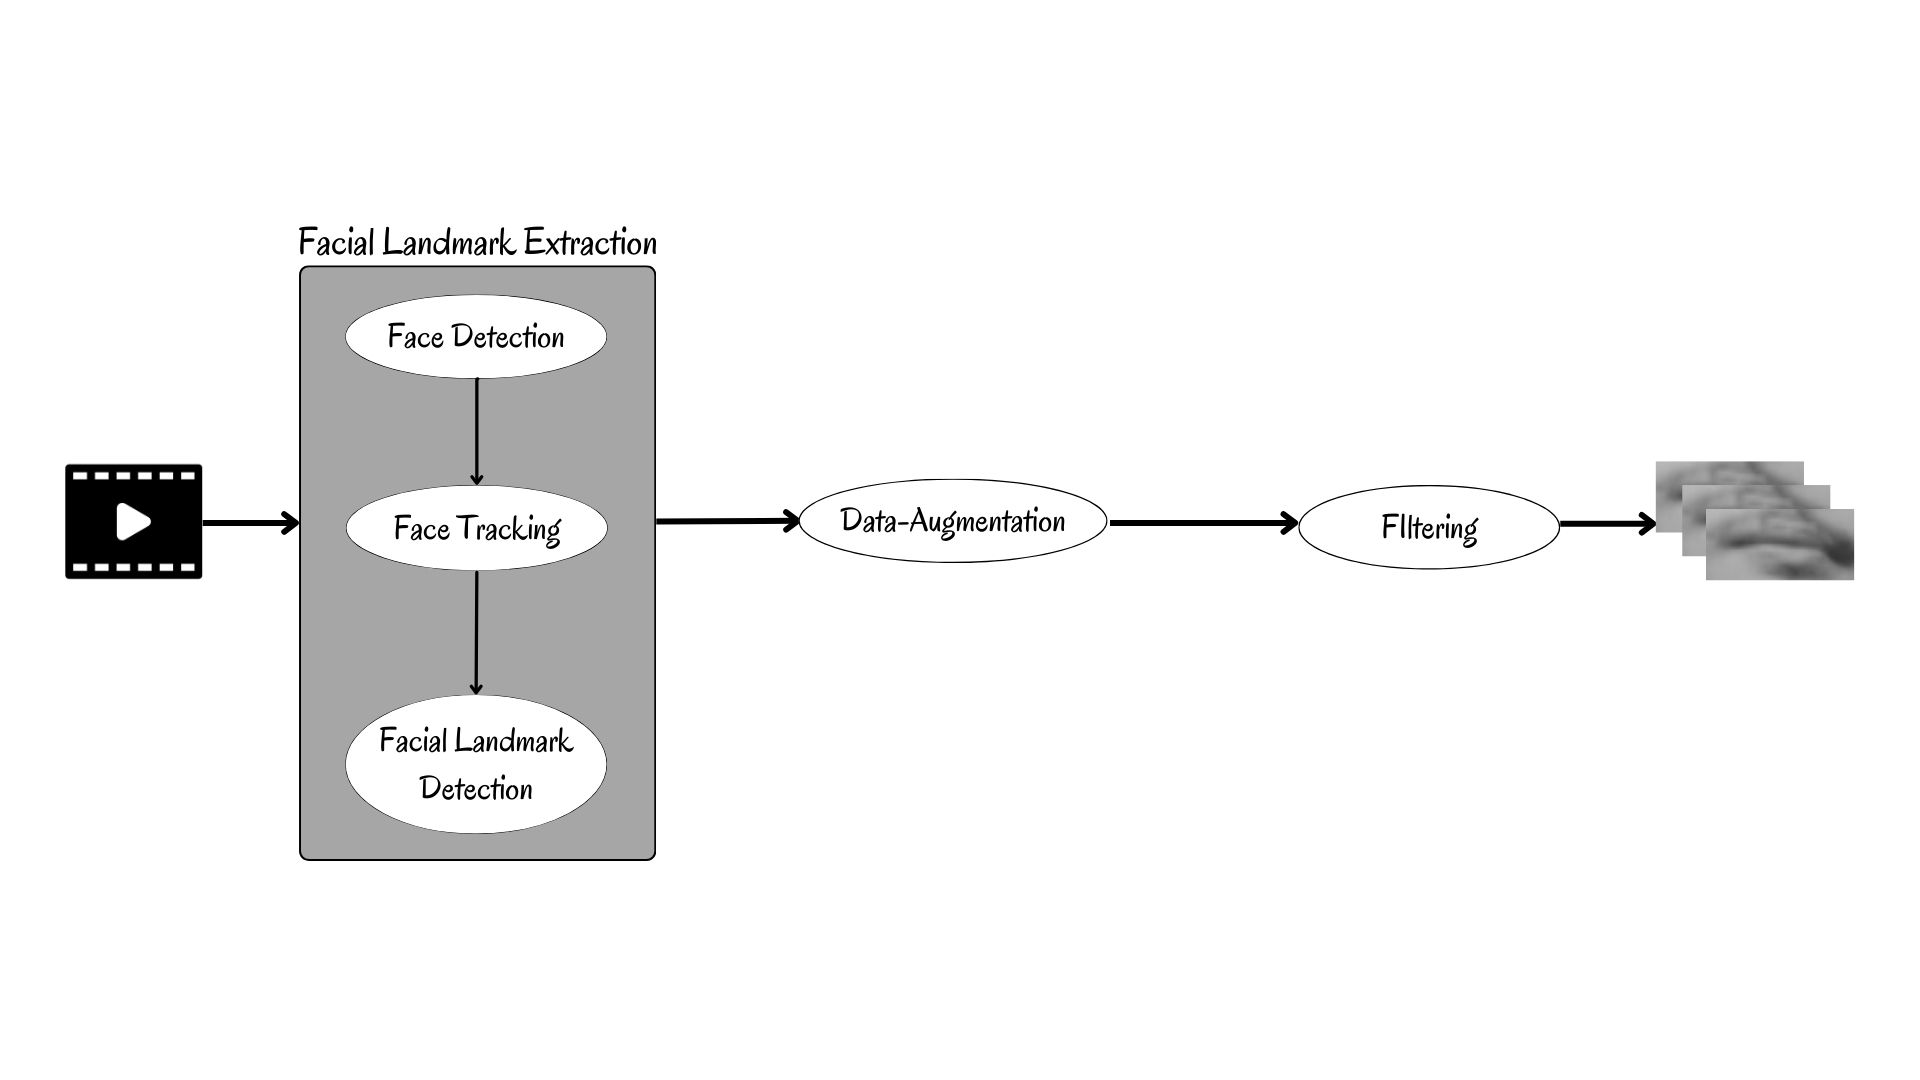
\includegraphics[width=\linewidth]{images/pre-processing.jpg}
	\caption{Pre-Processing}
	
	\end{figure}
	\pagebreak
	\item \textbf{Convolutional Neural Network (CNN):}
	\\In the lip reading project, Convolutional Neural Networks (CNNs) are utilized for spatial feature extraction from video frames capturing lip movements. CNNs excel in recognizing patterns within image data by employing convolutional layers and filters. The initial layers detect low-level features like edges and shapes, while deeper layers abstract higher-level representations related to the lips' spatial structures.The convolutional process involves sliding filters across the input image, enabling the network to identify spatial hierarchies and intricate patterns within the lip region. Pooling layers follow, reducing spatial dimensions and retaining essential information. These spatial features are crucial as they represent the distinctive visual cues of lip shapes and movements. By integrating CNNs into the lip reading system, the model becomes adept at discerning spatial intricacies, laying the foundation for subsequent processing stages that capture the temporal aspects of lip gestures using recurrent layers.
	
	
	\begin{figure}[h]
	\centering
	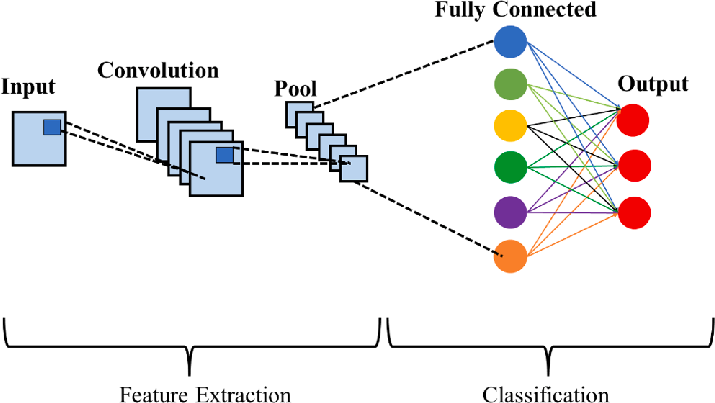
\includegraphics[scale=1.1]{images/CNN.png}
	\caption{Convolutional Neural Network}
	
	\end{figure}
	\item \textbf{Feature Extraction:}
	\\Feature extraction is a crucial step in the lip reading system, encompassing the identification and representation of relevant information from the spatial features obtained by the Convolutional Neural Network (CNN). This process aims to distill essential characteristics that best capture the discriminative aspects of lip movements for subsequent analysis.
In lip reading, features might include the shape, contour, and texture of the lips across frames. Feature extraction techniques often involve pooling layers that downsample spatial dimensions while retaining significant information. These features serve as a compact representation of the input data, emphasizing the most salient aspects relevant to lip dynamics. Moreover, temporal feature extraction follows, where recurrent layers like Long Short-Term Memory (LSTM) networks process the sequential nature of the features. This captures the dynamic evolution of lip movements over time. Efficient feature extraction is pivotal, as it enhances the model's ability to discern nuanced patterns in lip articulation, ultimately contributing to the accurate interpretation of spoken language from visual cues.
    
	\pagebreak
	\item \textbf{Recurrent Neural Network (RNN):}
	\\In the lip reading project, Recurrent Neural Networks (RNNs) are employed for temporal feature extraction, recognizing the sequential nature of lip movements captured in video frames. Unlike traditional neural networks, RNNs are equipped to maintain a memory of past inputs, making them well-suited for tasks where temporal dependencies play a crucial role. For lip reading, RNNs, particularly Long Short-Term Memory (LSTM) networks, are adept at learning and representing temporal patterns in the sequence of features obtained from the preceding Convolutional Neural Network (CNN) layers. LSTMs have memory cells that can selectively store and retrieve information over time, allowing the network to capture long-term dependencies in lip gestures.The RNN processes the sequence of spatial features, extracting temporal nuances such as the duration and timing of specific lip movements. By doing so, it enables the model to understand the dynamic evolution of lip articulation and enhances its capacity to decode spoken language accurately from visual cues. Temporal feature extraction with RNNs is vital for comprehending the temporal context inherent in lip reading tasks.
	\item \textbf{Long Short-Term Memory (LSTM) Cells}
	\\Long Short-Term Memory (LSTM) cells are a specialized type of recurrent neural network (RNN) architecture designed to address the challenges of capturing and learning long-range dependencies in sequential data. LSTMs play a crucial role in temporal feature extraction for tasks like lip reading.In the context of lip reading, LSTMs excel at modeling the temporal dynamics of lip movements over a sequence of video frames. Each LSTM cell contains a memory cell, input gate, forget gate, and output gate. The memory cell serves as a storage unit that can selectively retain or discard information over time. The input gate regulates the inflow of new information, while the forget gate manages the removal of unnecessary information from the memory cell. Finally, the output gate controls the information that is passed to the next time step or to the subsequent layers of the neural network. LSTM cells are particularly effective at mitigating the vanishing and exploding gradient problems often encountered in traditional RNNs, enabling them to capture and remember patterns in sequential data over extended time periods. In lip reading, LSTMs contribute to understanding the nuanced temporal relationships in lip gestures, facilitating accurate interpretation of spoken language from visual cues.

	\item \textbf{Temporal Feature Extraction:}
	\\Temporal feature extraction is a critical phase in the lip reading system, involving the capture and representation of dynamic patterns in sequential data, such as the temporal evolution of lip movements over video frames. In the context of lip reading, this process occurs after the spatial features are extracted using Convolutional Neural Networks (CNNs) and before the final classification stage. Temporal feature extraction is often facilitated by recurrent neural networks (RNNs), and specifically, Long Short-Term Memory (LSTM) cells. These specialized cells are designed to model and capture dependencies in sequential data, addressing issues like vanishing gradients and enabling the network to retain information over extended time intervals. During temporal feature extraction, the LSTM cells process the sequence of spatial features obtained from the lip regions across multiple frames. The memory cells within LSTMs maintain contextual information, allowing the model to discern the timing, duration, and patterns of specific lip movements. This step is crucial for understanding the temporal context of spoken language, providing the neural network with the ability to decode and interpret the phonetic information conveyed by the speaker's lips accurately.

	\item \textbf{Integration Layer:}
	\\The integration layer in a lip reading system serves as the point where spatial and temporal features are combined to create a comprehensive representation of lip movements. After Convolutional Neural Networks (CNNs) extract spatial features and Recurrent Neural Networks (RNNs), particularly Long Short-Term Memory (LSTM) cells, capture temporal dynamics, the integration layer merges these features. This layer harmonizes the spatial and temporal aspects, providing a unified and enriched representation of the lip gestures over time. The integrated features are then forwarded to subsequent layers for final processing and classification. The role of the integration layer is pivotal in ensuring that the model effectively combines both spatial and temporal information, optimizing its ability to interpret spoken language from visual cues accurately.
	
	\item \textbf{Fully Connected Layers:}
	\\Fully Connected Layers, also known as dense layers, are a crucial component in neural networks, including those used for lip reading. Following feature extraction and integration, fully connected layers process the concatenated or flattened features to make predictions or classifications. Each neuron in a fully connected layer is connected to every neuron in the previous layer, allowing the network to learn complex relationships and patterns. In the context of lip reading, these layers play a vital role in mapping the integrated spatial and temporal features to the output classes, facilitating the recognition of spoken words or phonemes. The weights and biases in these layers are adjusted during training to optimize the model's ability to accurately predict lip movements and, consequently, spoken language.

	\item \textbf{Output (Text Prediction):}
	\\The output in a lip reading system represents the final result or prediction made by the neural network based on the processed input data. In the context of lip reading, the output typically consists of transcriptions, phonemes, or textual representations of the spoken words or phrases. The output layer of the neural network produces a probability distribution over the possible classes or labels, and the final prediction is often determined by selecting the class with the highest probability. The goal is to accurately interpret the visual cues from lip movements and convert them into meaningful linguistic information. The output is then compared to the ground truth during training, and the model is optimized to minimize the difference between predicted and actual outputs using a suitable loss function.

\end{enumerate}